\section{Current state of our application}

We have use Sonarqube and codeclimate to analyze our code base. This section will describe the current state of our application, acording to the two analyze tools.

\subsection*{Codeclimate}

\begin{figure}[H]
	\centering
	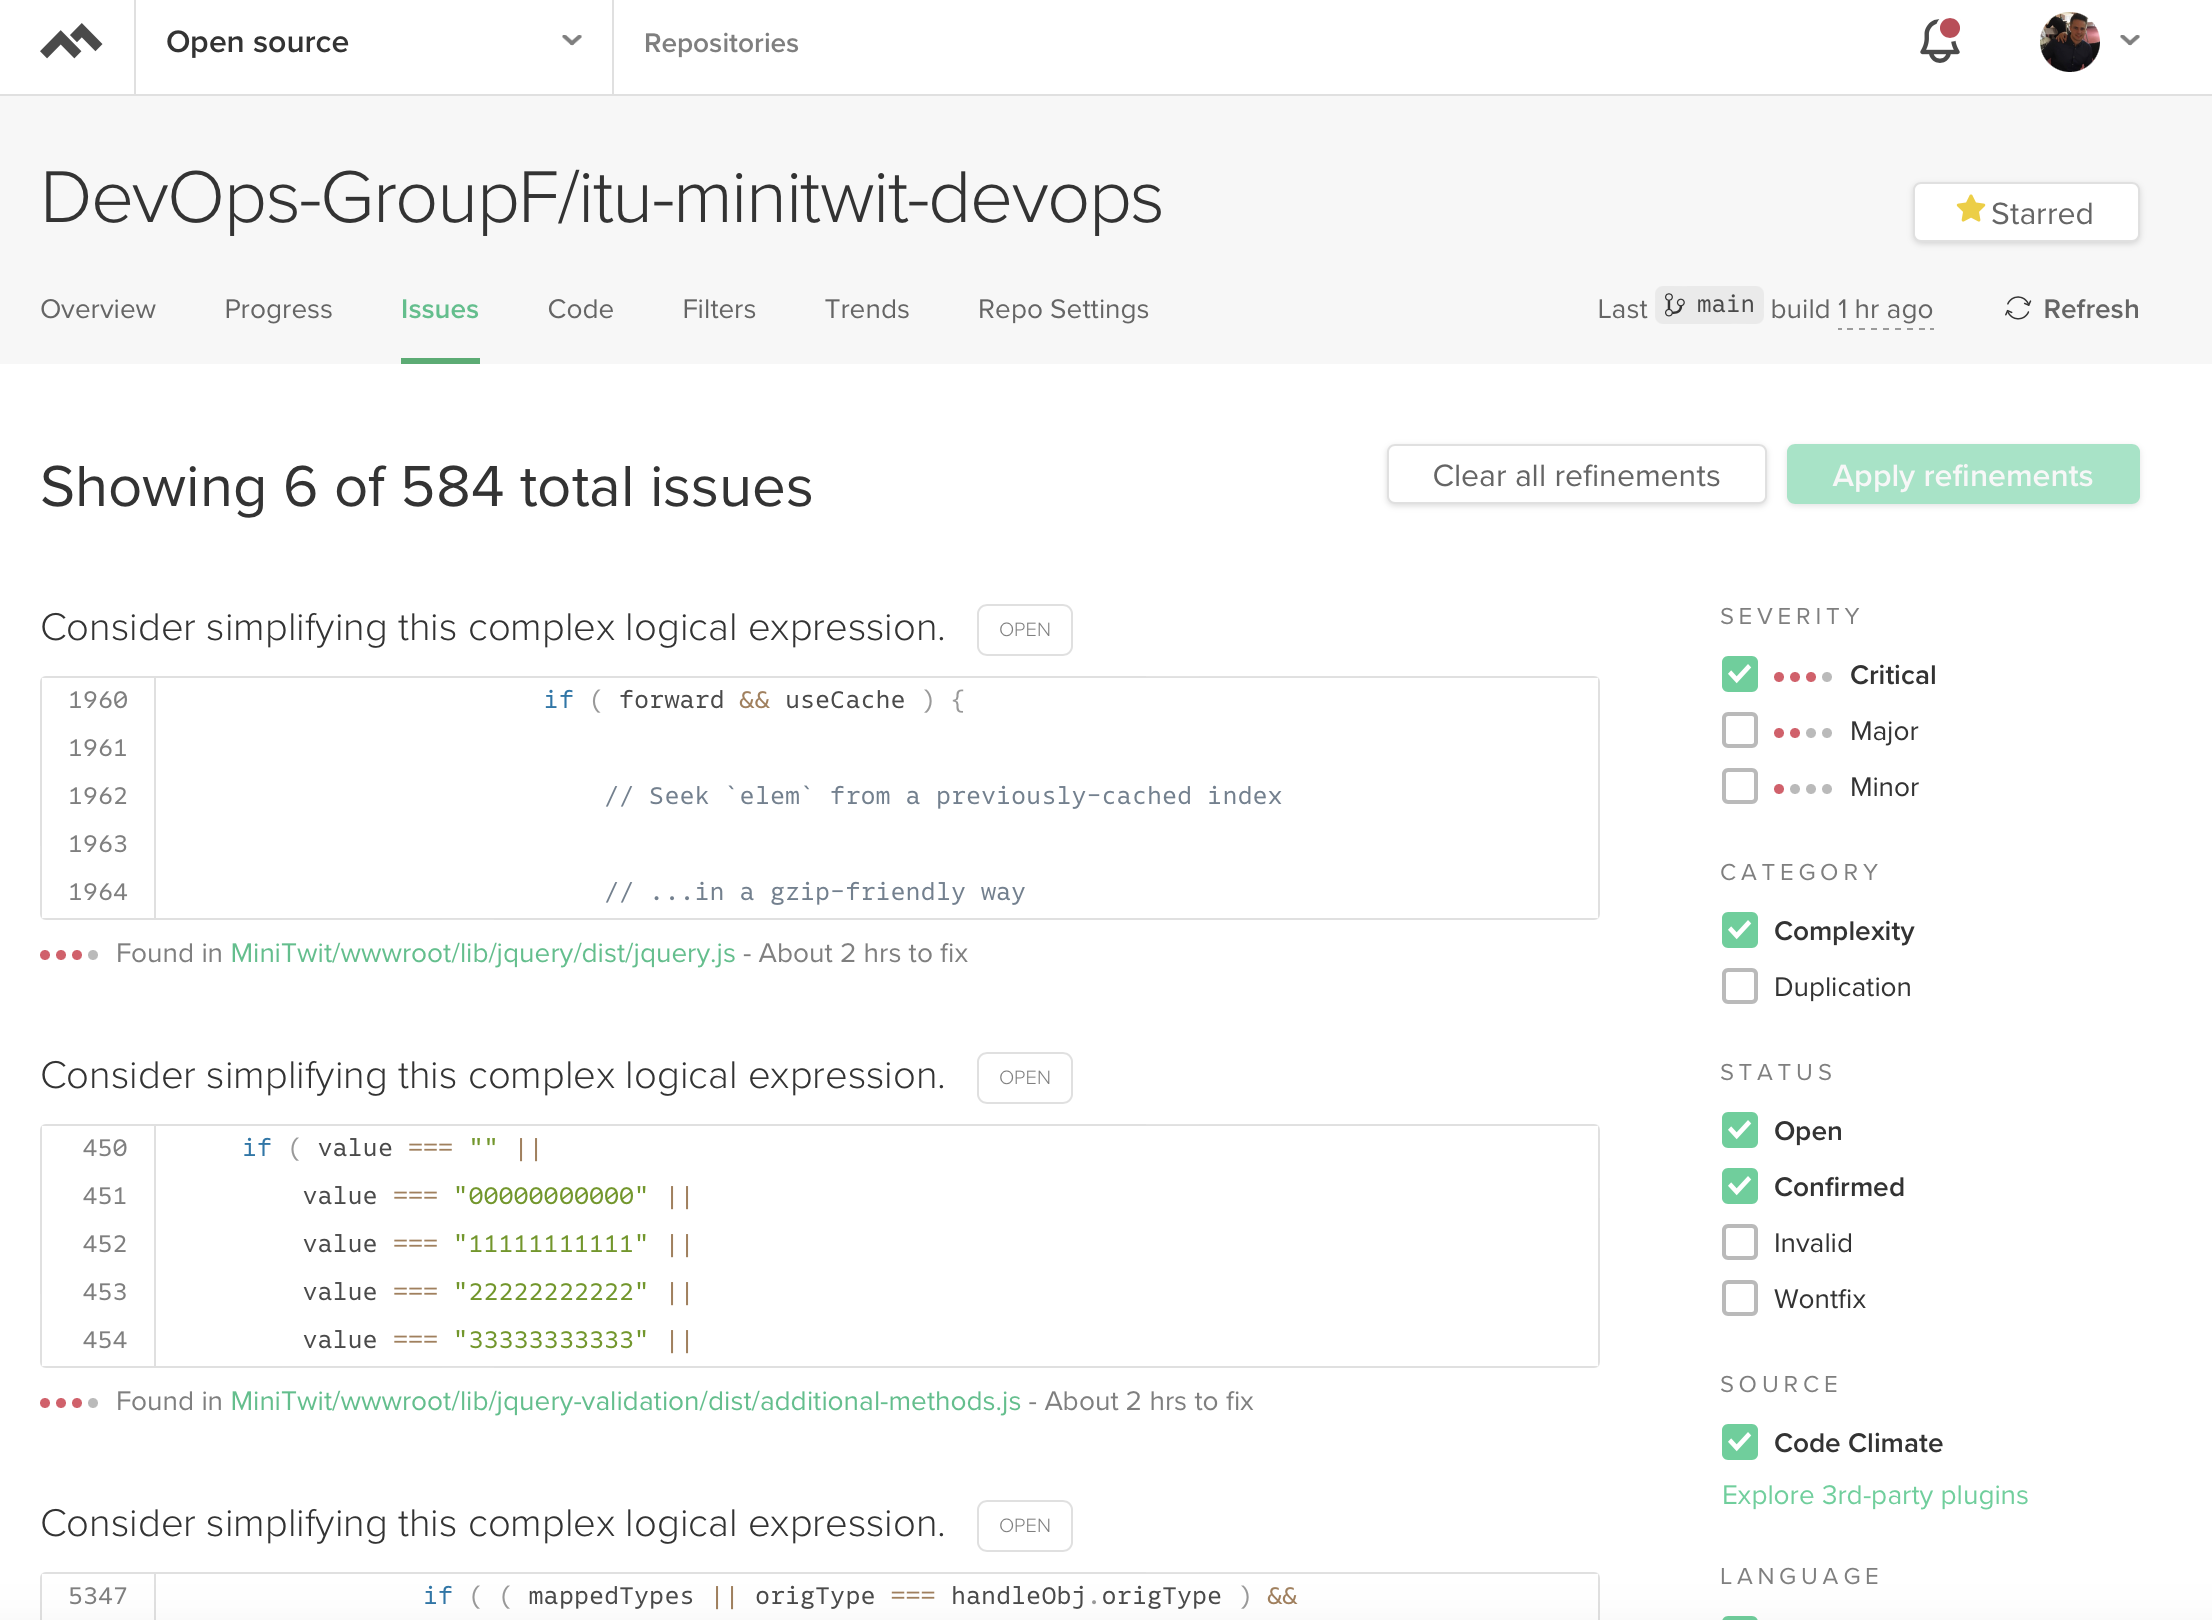
\includegraphics[width=0.75\textwidth]{codeclitemate.png}
	\caption{Code climate report}
	\label{fig:Code climate}
\end{figure}

Codeclimate general reports 323 code smells, and 261 duplication. Mostly of these is from the javascript lib we are using, for some reason even try to filter code, so only \texttt{C\#} code is shown, it still include it. Also it was also possible to filter critical issues, here were 6 found, but related to our used third party javascript library jquery. %So nothing we can do here. 

\subsection*{Sonarqube}
Sunarqube report several issues. Mostly it report security issues, because we are logging to much in our application, which could cause security issues.
\begin{figure}[H]
	\centering
	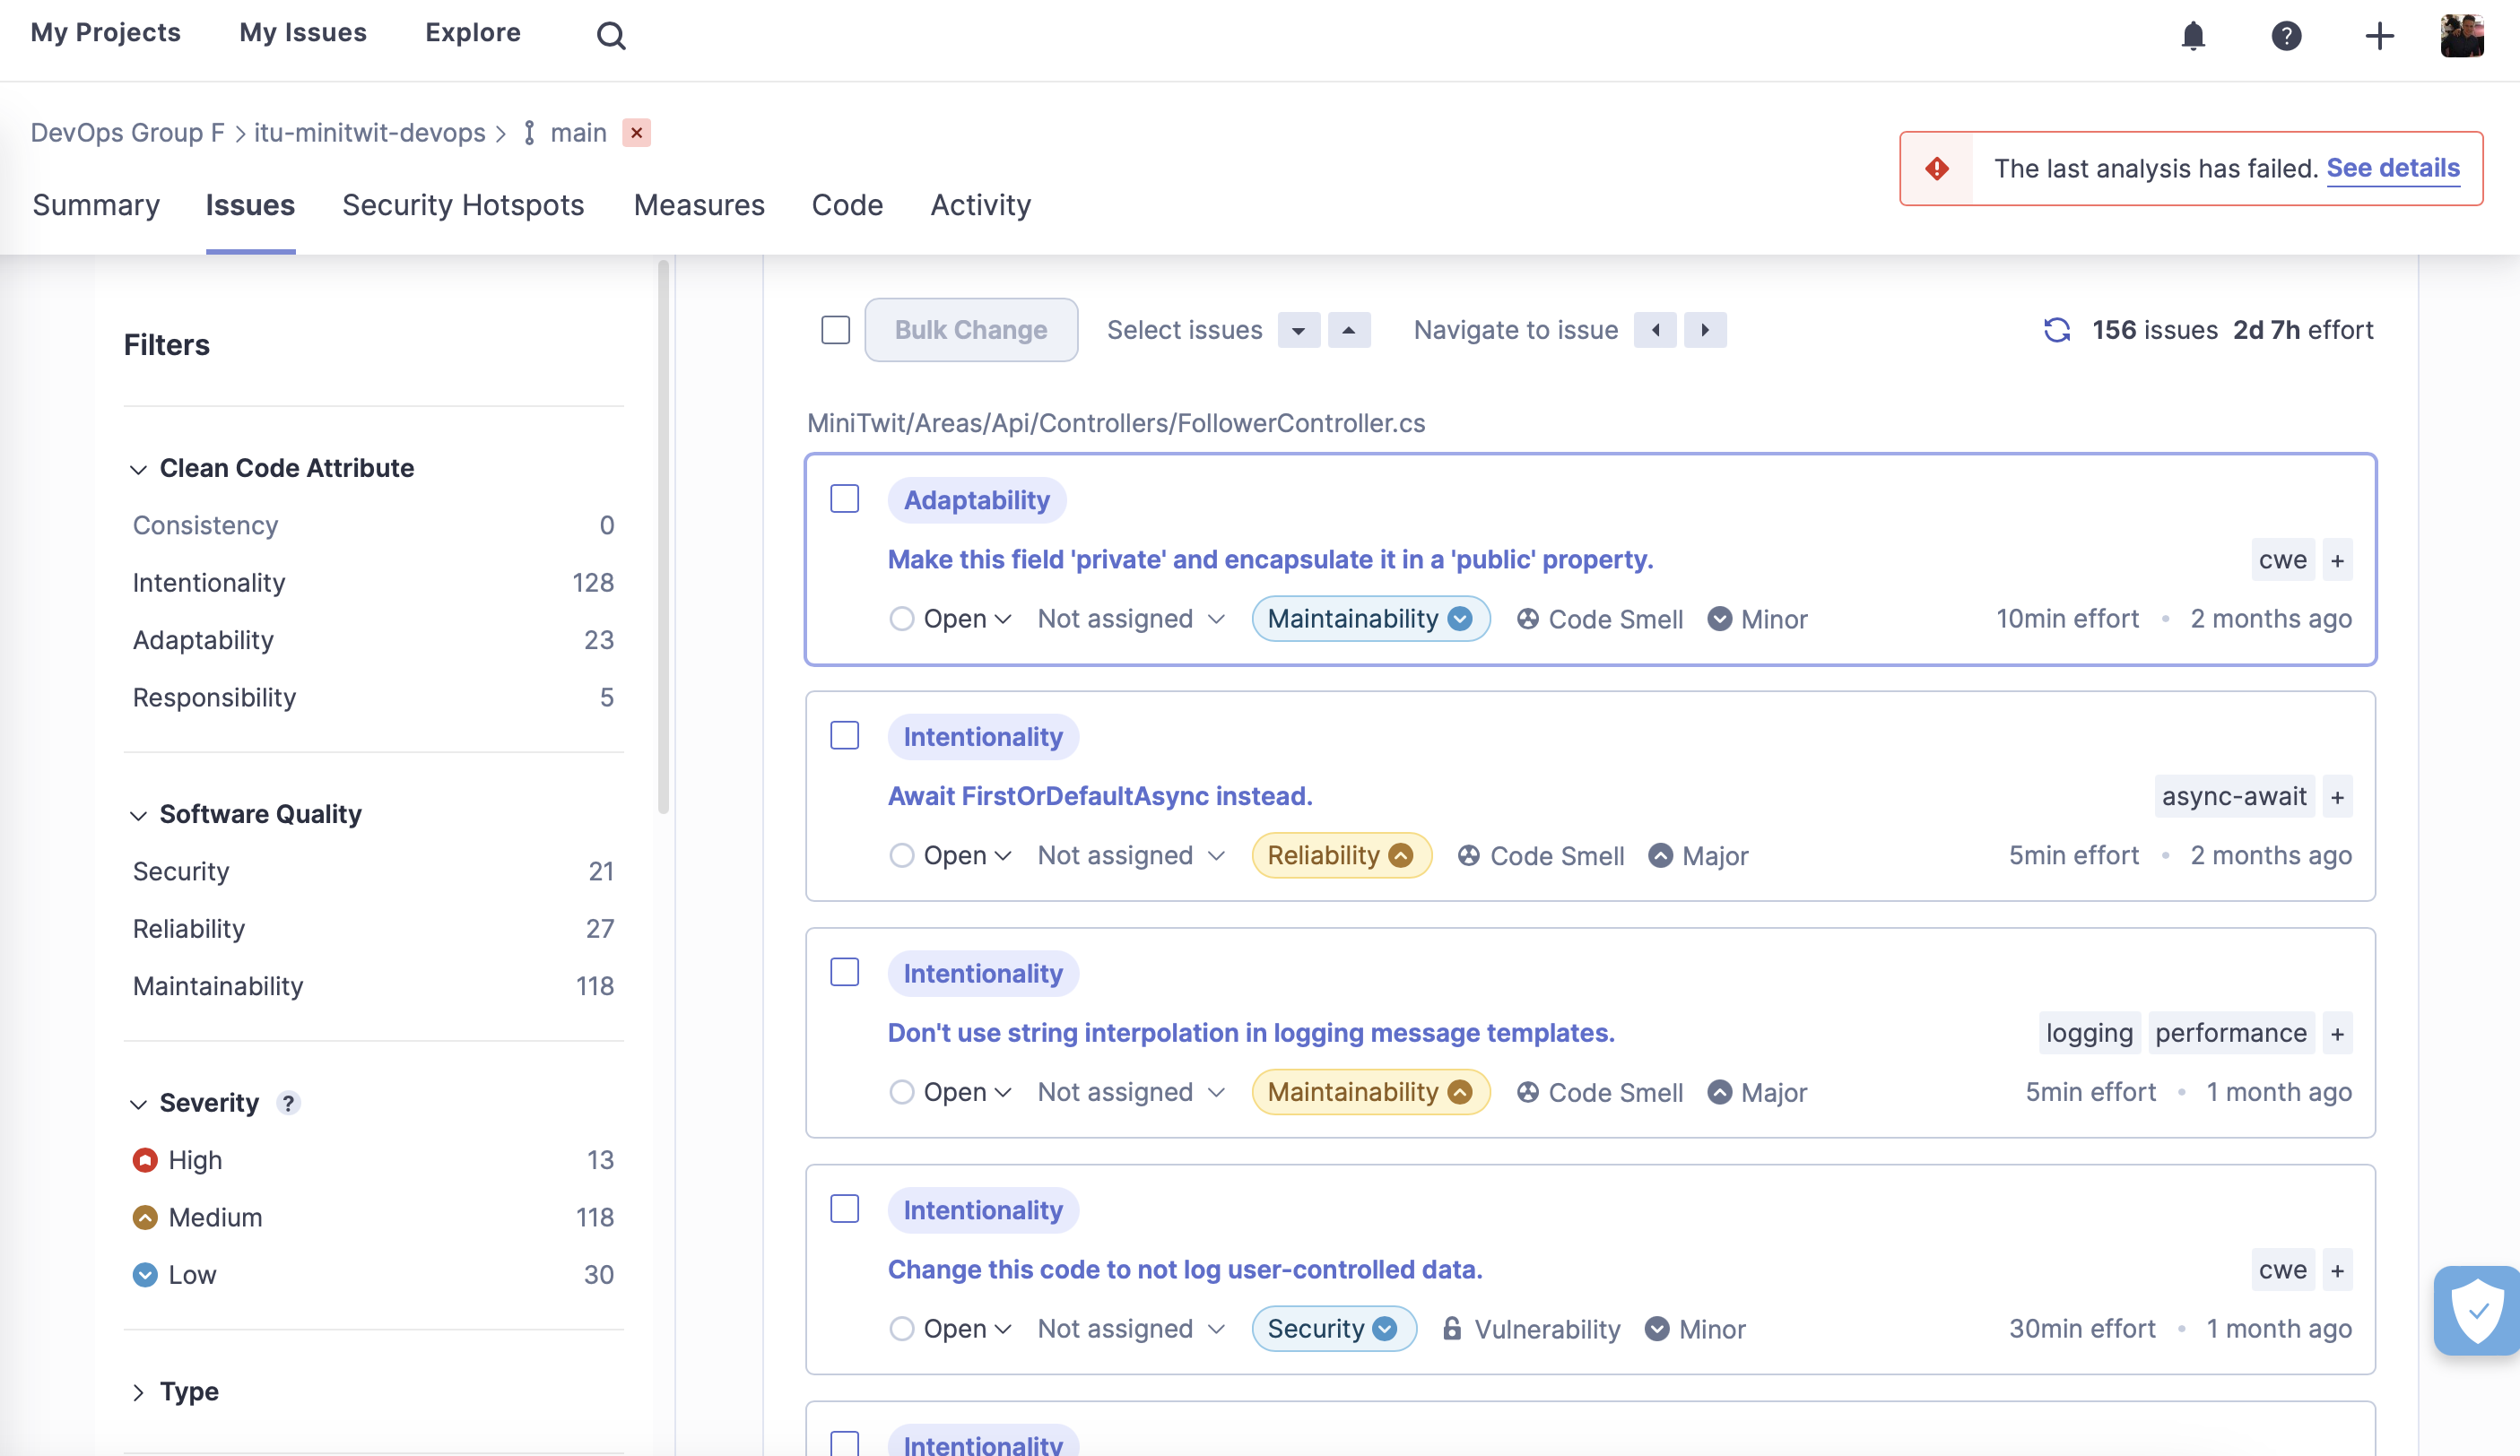
\includegraphics[width=0.75\textwidth]{sonarqube.png}
	\caption{Sonarqube report}
	\label{fig:Sonarqube}
\end{figure}
